\documentclass[main.tex]{subfiles}

\begin{document}
\section{Results}
\subsection{Test Data}
\begin{frame}{Test Data}
	\begin{itemize}
		\item { 
			We generate 2 random datasets for testing and evaluating different approaches:
			\begin{itemize}
				\item Full set: 10 instances within an area of size 1000x1000, N = 200, M = 200, Y = 20. This is identical to the configuration used by Yuan et al.
				\item Small set: 10 instances within an area of size 200x200, N = 40, M = 40, Y = 4. This is a smaller set used for quick testing. Due to time constraints, we will report our results mostly on this dataset.
			\end{itemize}
		}
	\end{itemize}
\end{frame}

\subsection{Experiment Setup}
\begin{frame}{Experiment Setup}
	\begin{itemize}
		\item Yuan's heuristics are only run once as they are deterministic.
		\item {
			GA configurations:
			\begin{itemize}
				\item Maximum iterations: 10,000
				\item Early stop after 40 generations without any improvements.
				\item Population size: 70
				\item Crossover ratio: 80\%
				\item Mutation ratio: 5\%
			\end{itemize}
		}
		\item Results for GA are measured in 20 runs for each input set.
	\end{itemize}
\end{frame}

\subsection{Experiment Results}
\begin{frame}{Experiment Results}{GA w/ MFP}
\begin{table}[]
\centering
\resizebox{\textwidth}{!}{
\begin{tabular}{|c|c|c|c|c|c|c|c|c|}
\hline
\diagbox[width=6em]{Test}{Alg.} & \multicolumn{2}{c|}{\textbf{LU1/LB3}} & \multicolumn{2}{c|}{\textbf{LU2/LB3}} & \multicolumn{3}{c|}{\textbf{GA w/ MFP}} \\ \hline
\multicolumn{1}{|l|}{}          & t (ms)         & Loss        & t (ms)           & Loss           & Avg. t (ms)  & Avg. Loss  & Min Loss \\ \hline
\textbf{1} & 62.64 & 256.73 & 2321.90 & 271.43 & 372489.13 & 237.86 & \textbf{236.49} \\ \hline
\textbf{2} & 47.36 & 255.43 & 2292.88 & 268.88 & 388895.01 & 237.52 & \textbf{234.88} \\ \hline
\textbf{3} & 51.12 & 256.90 & 2306.35 & 266.26 & 328476.59 & 238.99 & \textbf{236.65} \\ \hline
\textbf{4} & 49.88 & 251.14 & 2434.52 & 273.09 & 310610.72 & 242.87 & \textbf{242.60} \\ \hline
\textbf{5} & 47.61 & 257.40 & 2366.93 & 280.79 & 312059.40 & 238.01 & \textbf{237.99} \\ \hline
\textbf{6} & 50.02 & 261.66 & 2384.48 & 262.81 & 307055.92 & 241.15 & \textbf{241.11} \\ \hline
\textbf{7} & 94.37 & 257.11 & 2367.25 & 274.89 & 388824.39 & 240.31 & \textbf{239.14} \\ \hline
\textbf{8} & 52.71 & 247.77 & 2393.78 & 277.49 & 329.41753 & 237.05 & \textbf{235.47} \\ \hline
\textbf{9} & 49.10 & 258.66 & 2903.16 & 276.62 & 329310.96 & 239.14 & \textbf{234.88} \\ \hline
\textbf{10} & 51.29 & 259.50 & 2897.00 & 272.32 & 328773.05 & 239.14 & \textbf{234.88} \\ \hline
\end{tabular}}
\caption{Results on Small Dataset}
\end{table}
\end{frame}

\begin{frame}{Experiment Results}{GA w/ Clustering}
\begin{table}[]
\centering
\resizebox{\textwidth}{!}{
\begin{tabular}{|c|c|c|c|c|c|c|c|c|}
\hline
\diagbox[width=6em]{Test}{Alg.} & \multicolumn{2}{c|}{\textbf{LU1/LB3}} & \multicolumn{2}{c|}{\textbf{LU2/LB3}} & \multicolumn{3}{c|}{\textbf{GA w/ Clustering}} \\ \hline
\multicolumn{1}{|l|}{}          & t (ms)         & Loss        & t (ms)           & Loss           & Avg. t (ms)  & Avg. Loss  & Min Loss \\ \hline
\textbf{1} & 62.64 & 256.73 & 2321.90 & 271.43 & 179013.99 & 248.00 & \textbf{240.82} \\ \hline
\textbf{2} & 47.36 & 255.43 & 2292.88 & 268.88 & 187870.14 & 248.81 & \textbf{239.20} \\ \hline
\textbf{3} & 51.12 & 256.90 & 2306.35 & 266.26 & 180623.50 & 249.18 & \textbf{242.89} \\ \hline
\textbf{4} & 49.88 & 251.14 & 2434.52 & 273.09 & 199641.77 & 249.95 & \textbf{241.36} \\ \hline
\textbf{5} & 47.61 & 257.40 & 2366.93 & 280.79 & 214119.68 & 247.97 & \textbf{242.99} \\ \hline
\textbf{6} & 50.02 & 261.66 & 2384.48 & 262.81 & 206661.67 & 252.89 & \textbf{243.13} \\ \hline
\textbf{7} & 94.37 & 257.11 & 2367.25 & 274.89 & 222644.89 & 251.03 & \textbf{247.45} \\ \hline
\textbf{8} & 52.71 & \textbf{247.77} & 2393.78 & 277.49 & 200350.64 & 250.34 & \textbf{245.50} \\ \hline
\textbf{9} & 49.10 & 258.66 & 2903.16 & 276.62 & 195602.57 & 243.20 & \textbf{238.84} \\ \hline
\textbf{10} & 51.29 & 259.50 & 2897.00 & 272.32 & 196454.75 & 248.76 & \textbf{241.63} \\ \hline
\end{tabular}}
\caption{Results on Small Dataset}
\end{table}
\end{frame}

\begin{frame}{Example Result}{Heuristics}
	\begin{center}
		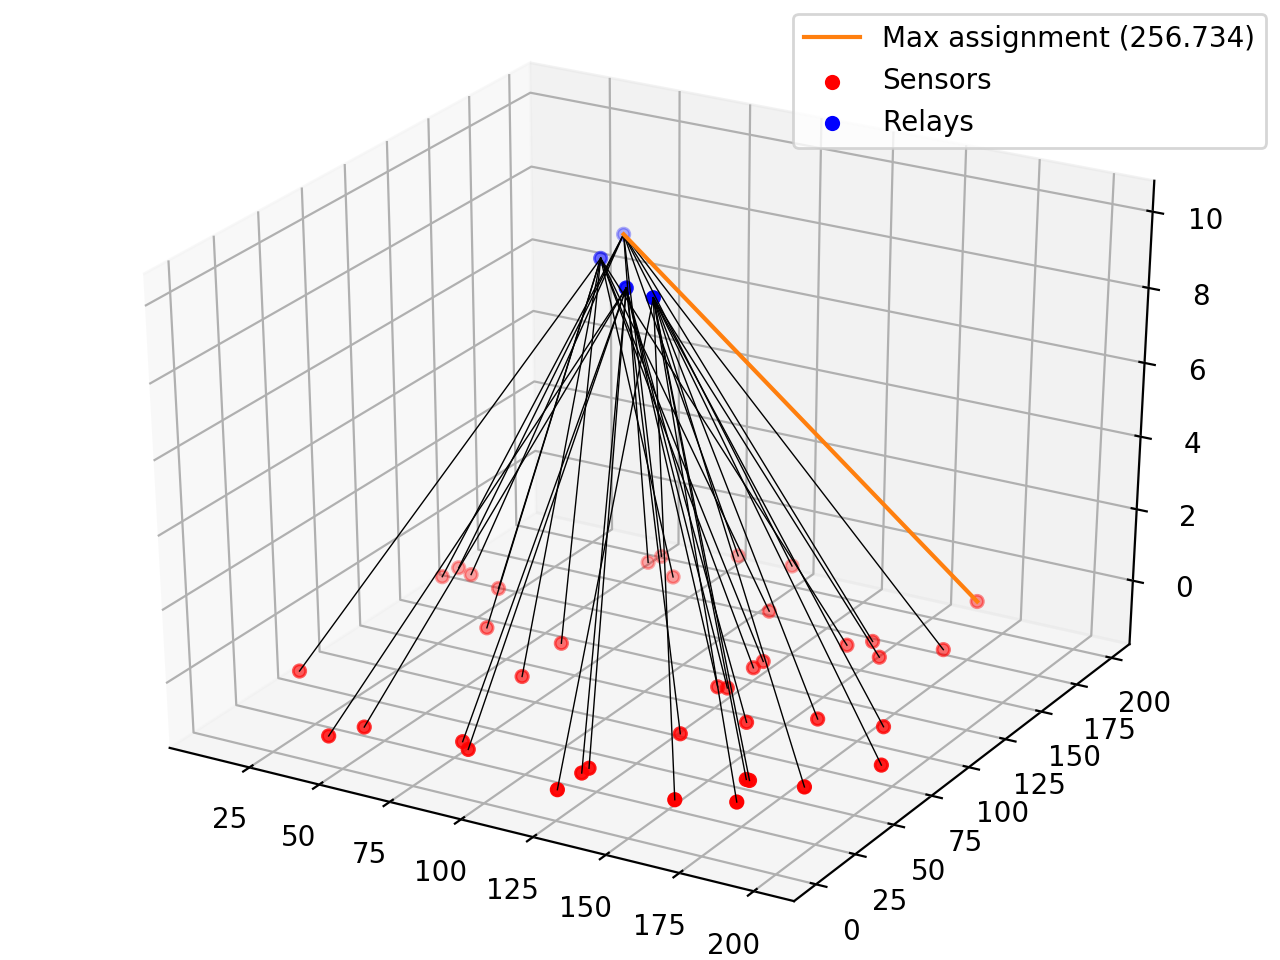
\includegraphics[scale=0.5]{YuanExample.png}
		\captionof{figure}{Example output of Yuan's heuristics}
	\end{center}
\end{frame}

\begin{frame}{Example Result}{GA w/ MFP}
	\begin{center}
		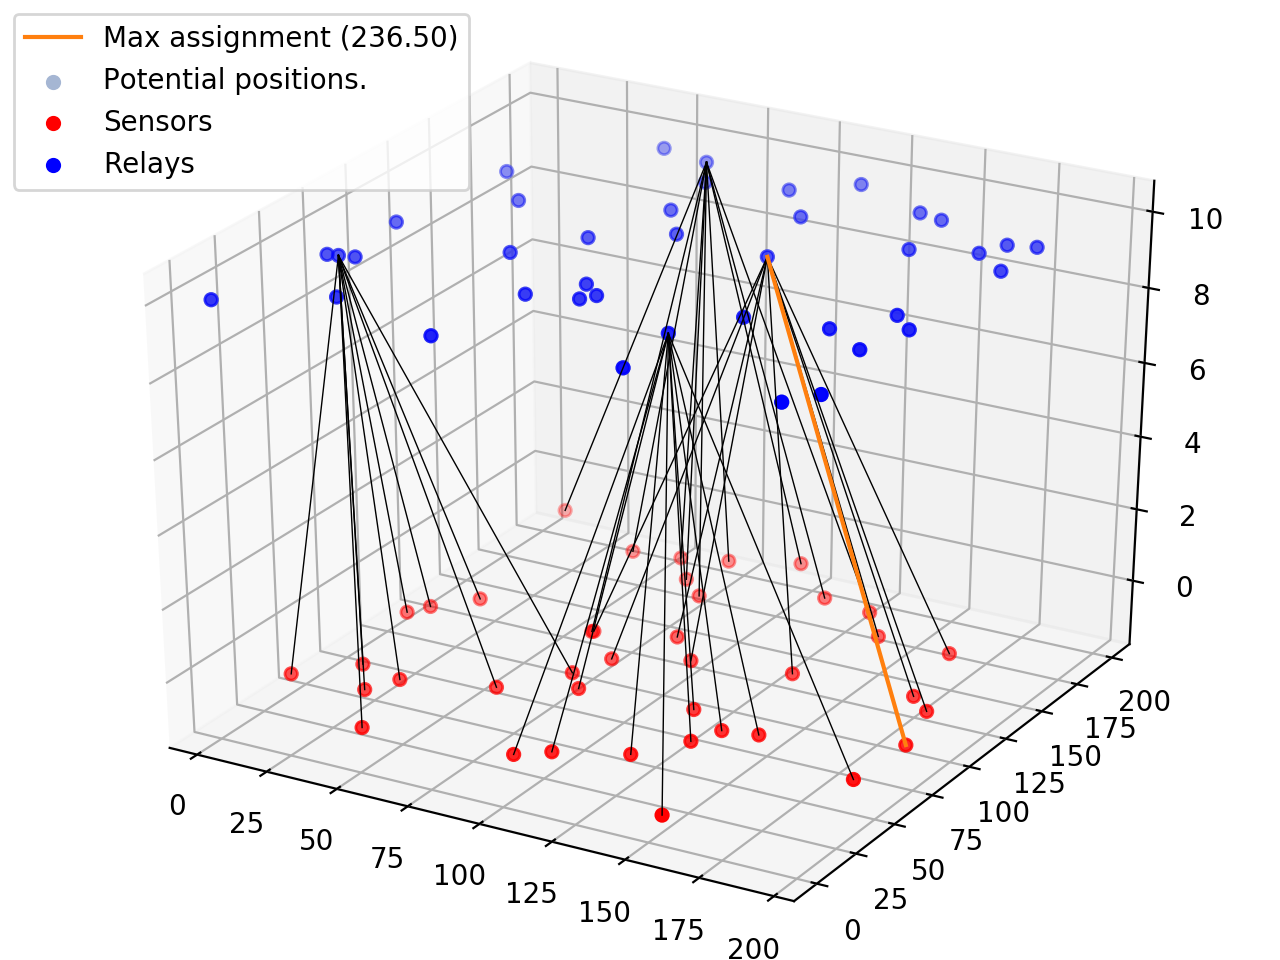
\includegraphics[scale=0.18]{Prop1Example.png}
		\captionof{figure}{Example output of MFP GA}
	\end{center}
\end{frame}

\begin{frame}{Example Result}{GA w/ Clustering}
	\begin{center}
		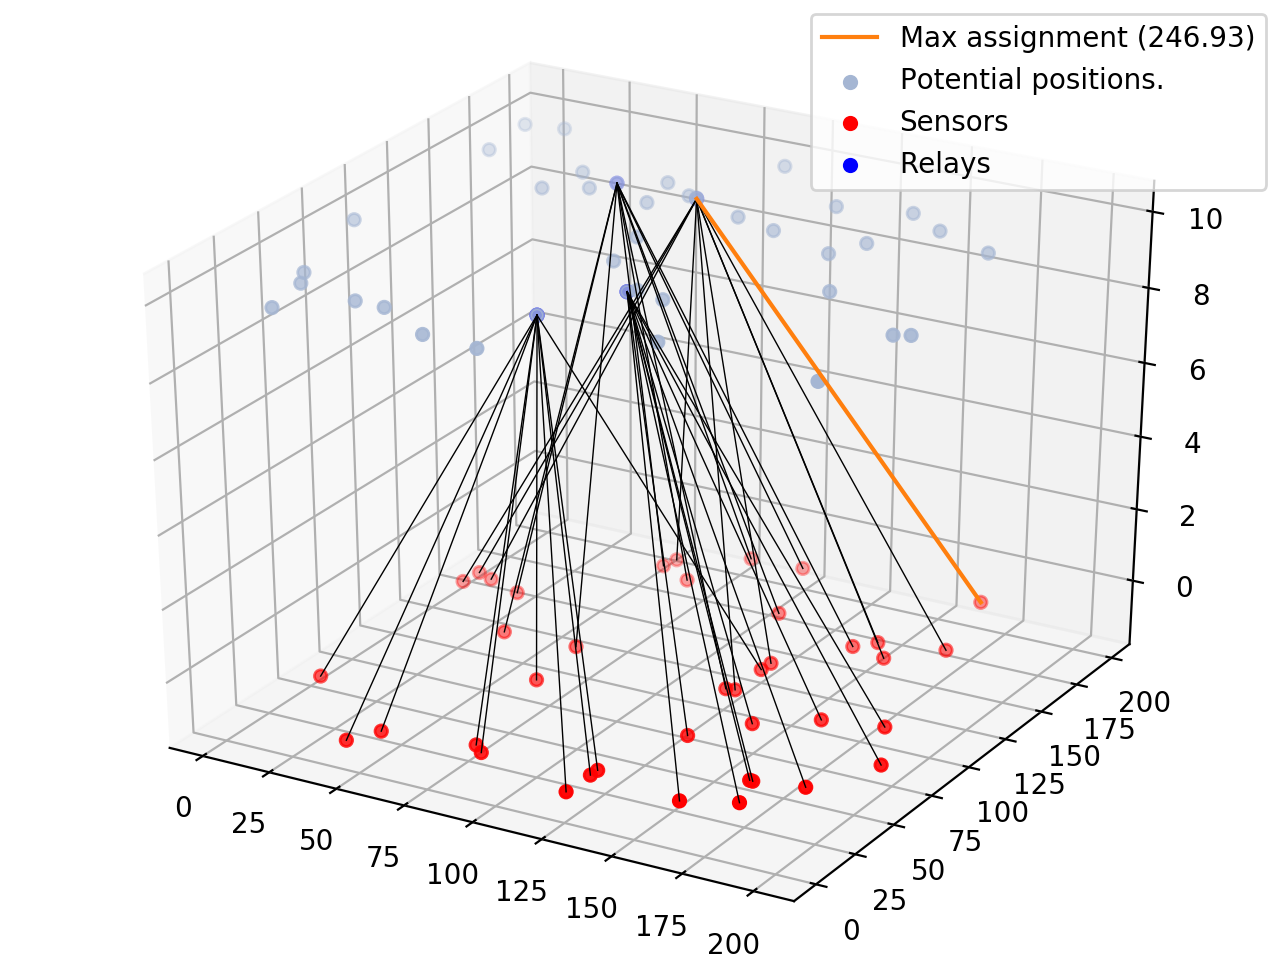
\includegraphics[scale=0.5]{Prop2Example.png}
		\captionof{figure}{Example output of Cluster GA}
	\end{center}
\end{frame}

\end{document}
